\documentclass[journal,12pt,twocolumn]{IEEEtran}
\usepackage{setspace}
\usepackage{gensymb}
\usepackage{xcolor}
\usepackage{caption}
\singlespacing
\usepackage{siunitx}
\usepackage[cmex10]{amsmath}
\usepackage{mathtools}
\usepackage{hyperref}
\usepackage{amsthm}
\usepackage{mathrsfs}
\usepackage{txfonts}
\usepackage{stfloats}
\usepackage{cite}
\usepackage{cases}
\usepackage{subfig}
\usepackage{longtable}
\usepackage{multirow}
\usepackage{enumitem}
\usepackage{bm}
\usepackage{mathtools}
\usepackage{listings}
\usepackage{tikz}
\usetikzlibrary{shapes,arrows,positioning}
\usepackage{circuitikz}
\renewcommand{\vec}[1]{\boldsymbol{\mathbf{#1}}}
\DeclareMathOperator*{\Res}{Res}
\renewcommand\thesection{\arabic{section}}
\renewcommand\thesubsection{\thesection.\arabic{subsection}}
\renewcommand\thesubsubsection{\thesubsection.\arabic{subsubsection}}

\renewcommand\thesectiondis{\arabic{section}}
\renewcommand\thesubsectiondis{\thesectiondis.\arabic{subsection}}
\renewcommand\thesubsubsectiondis{\thesubsectiondis.\arabic{subsubsection}}
\hyphenation{op-tical net-works semi-conduc-tor}

\lstset{
language=Python,
frame=single, 
breaklines=true,
columns=fullflexible
}
\begin{document}
\theoremstyle{definition}
\newtheorem{theorem}{Theorem}[section]
\newtheorem{problem}{Problem}
\newtheorem{proposition}{Proposition}[section]
\newtheorem{lemma}{Lemma}[section]
\newtheorem{corollary}[theorem]{Corollary}
\newtheorem{example}{Example}[section]
\newtheorem{definition}{Definition}[section]
\newcommand{\BEQA}{\begin{eqnarray}}
        \newcommand{\EEQA}{\end{eqnarray}}
\newcommand{\define}{\stackrel{\triangle}{=}}
\newcommand{\myvec}[1]{\ensuremath{\begin{pmatrix}#1\end{pmatrix}}}
\newcommand{\mydet}[1]{\ensuremath{\begin{vmatrix}#1\end{vmatrix}}}
\bibliographystyle{IEEEtran}
\providecommand{\nCr}[2]{\,^{#1}C_{#2}} % nCr
\providecommand{\nPr}[2]{\,^{#1}P_{#2}} % nPr
\providecommand{\mbf}{\mathbf}
\providecommand{\pr}[1]{\ensuremath{\Pr\left(#1\right)}}
\providecommand{\qfunc}[1]{\ensuremath{Q\left(#1\right)}}
\providecommand{\sbrak}[1]{\ensuremath{{}\left[#1\right]}}
\providecommand{\lsbrak}[1]{\ensuremath{{}\left[#1\right.}}
\providecommand{\rsbrak}[1]{\ensuremath{{}\left.#1\right]}}
\providecommand{\brak}[1]{\ensuremath{\left(#1\right)}}
\providecommand{\lbrak}[1]{\ensuremath{\left(#1\right.}}
\providecommand{\rbrak}[1]{\ensuremath{\left.#1\right)}}
\providecommand{\cbrak}[1]{\ensuremath{\left\{#1\right\}}}
\providecommand{\lcbrak}[1]{\ensuremath{\left\{#1\right.}}
\providecommand{\rcbrak}[1]{\ensuremath{\left.#1\right\}}}
\theoremstyle{remark}
\newtheorem{rem}{Remark}
\newcommand{\sgn}{\mathop{\mathrm{sgn}}}
\newcommand{\rect}{\mathop{\mathrm{rect}}}
\newcommand{\sinc}{\mathop{\mathrm{sinc}}}
\providecommand{\abs}[1]{\left\vert#1\right\vert}
\providecommand{\res}[1]{\Res\displaylimits_{#1}}
\providecommand{\norm}[1]{\lVert#1\rVert}
\providecommand{\mtx}[1]{\mathbf{#1}}
\providecommand{\mean}[1]{E\left[ #1 \right]}
\providecommand{\fourier}{\overset{\mathcal{F}}{ \rightleftharpoons}}
\providecommand{\ztrans}{\overset{\mathcal{Z}}{ \rightleftharpoons}}
\providecommand{\system}[1]{\overset{\mathcal{#1}}{ \longleftrightarrow}}
\newcommand{\solution}{\noindent \textbf{Solution: }}
\providecommand{\dec}[2]{\ensuremath{\overset{#1}{\underset{#2}{\gtrless}}}}
\let\StandardTheFigure\thefigure
\def\putbox#1#2#3{\makebox[0in][l]{\makebox[#1][l]{}\raisebox{\baselineskip}[0in][0in]{\raisebox{#2}[0in][0in]{#3}}}}
\def\rightbox#1{\makebox[0in][r]{#1}}
\def\centbox#1{\makebox[0in]{#1}}
\def\topbox#1{\raisebox{-\baselineskip}[0in][0in]{#1}}
\def\midbox#1{\raisebox{-0.5\baselineskip}[0in][0in]{#1}}

\vspace{3cm}
\title{11.11.5.3}
\author{Lokesh Surana}
\maketitle
\section*{Class 11, Chapter 11, Exercise 5.3}

Q. The cable of a uniformly loaded suspension bridge hangs in the form of a parabola. The roadway which is horizontal and 100 m long is supported by vertical wires attached to the cable, the longest wire being 30 m and the shortest being 6 m. Find the length of a supporting wire attached to the roadway 18 m from the middle.

\solution
Uniformly loaded suspension bridge cable hangs in the form of a parabola facing upwards.
The length of cable,
\begin{align}
    AB = 100m
\end{align}
Let's assume that vertex of this parabolic setup is $\myvec{0\\0}$.

This will give us a setup similar to below figure,
\begin{figure}[!htb]
    \centering
    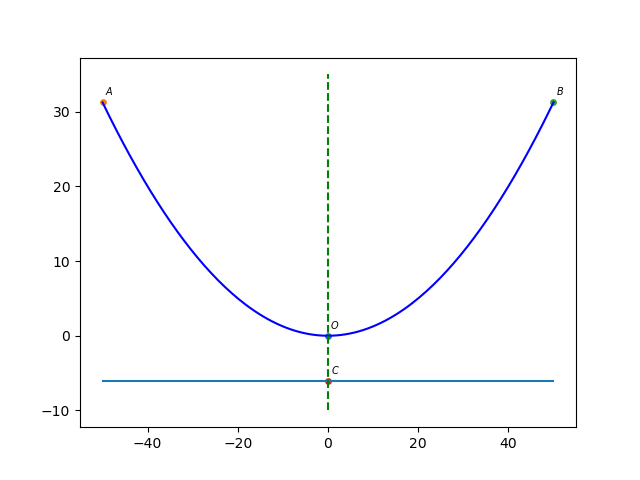
\includegraphics[width=\columnwidth]{figs/1.png}
    \caption{Representation of parabola with vertex at origin.}
    \label{fig:Cable}
\end{figure}

Here A and B are the points on the parabola where the cable is attached to the roadway, i.e. longest wire is attached at this points. And vertex of parabola O is point where shortest wire is attached, which is 6m from the ground.
With the assumption of point $O$ being $\myvec{0\\0}$, we'll get Point $A = \myvec{50\\24}$ and Point $B = \myvec{-50\\24}$.  

The generic equation of conic is
\begin{align}
    \label{eq:1} g\brak{\vec{x}} = \vec{x}^T\vec{V}\vec{x} + 2\vec{u}^T\vec{x} + f = 0 
\end{align}

Point $\myvec{0\\0}$ is on conic, so
\begin{align}
    \implies f = 0
\end{align}

As conic is upward facing parabola,
\begin{align}
    \vec{V} = \myvec{1&0\\0&0}.
\end{align}

As points A and B are on parabola
\begin{align}
    \implies \myvec{50&24}\myvec{1&0\\0&0}\myvec{50\\24} + 2\vec{u}^\top\myvec{50\\24} &= 0\\
    \label{eq:u1} \implies \vec{u}^{\top}\myvec{50\\24} &= -1250
\end{align}
and
\begin{align}
    \implies \myvec{-50&24}\myvec{1&0\\0&0}\myvec{-50\\24} + 2\vec{u}^\top\myvec{-50\\24} &= 0\\
    \label{eq:u2} \implies \vec{u}^{\top}\myvec{-50\\24} &= -1250
\end{align}

From \eqref{eq:u1} and \eqref{eq:u2}, we get
\begin{align}
    \vec{u}^\top\myvec{50&-50\\24&24} &= \myvec{1250&-1250}\\
    \implies \vec{u} &= \myvec{0\\-\frac{625}{12}}
\end{align} 

we get parabola
\begin{align}
    \label{eq:parab1} \vec{x}^\top\myvec{1&0\\0&0}\vec{x} + 2\myvec{0\\-\frac{625}{12}\vec{x}} &= 0 
\end{align}

At a point $18 m$ from middle, let's call it $D = \myvec{18\\x_2}$.
\begin{align}
    \myvec{18&x_2}\myvec{1&0\\0&0}\myvec{18\\x_2} + 2\myvec{0\\-\frac{625}{12}}\myvec{18\\x_2} &= 0\\
    \implies x_2 = 3.3 
\end{align}

$\implies$ Length of a supporting wire attached to the roadway $18 m$ from the middle is 
\begin{align}
    = x_2 + 6 = 3.3 + 6 = 9.3 m    
\end{align}

\begin{figure}[!htb]
    \centering
    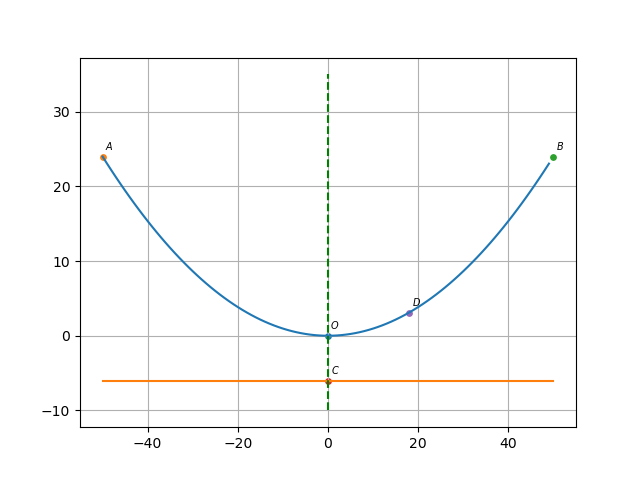
\includegraphics[width=\columnwidth]{figs/parabola.png}
    \caption{Parabola}
    \label{fig:parabola}
\end{figure}

\end{document}